\documentclass[10pt]{article}
\usepackage[a4paper, left=1.5cm, right=1.5cm, top=3.5cm]{geometry}
\usepackage[ngerman]{babel}
\usepackage[]{graphicx}
\usepackage{multicol}
\usepackage{amssymb}
\usepackage{inputenc}
\usepackage{breqn}
\usepackage{titlesec}
\usepackage{wrapfig}
\usepackage{blindtext}
\usepackage{lipsum}
\usepackage{caption}
\usepackage{listings}
\usepackage{fancyhdr}
\usepackage{nopageno}
\usepackage{authblk}
\usepackage{amsmath}
\usepackage{mathtools}
\usepackage{bm}
\usepackage[ISO]{diffcoeff}
\usepackage{xcolor}
\usepackage{csquotes}
\usepackage{siunitx}
\usepackage{circuitikz}
\usepackage{biblatex}
\fancyhf[]{}

\addbibresource{latex.bib}

\newenvironment{Figure}
  {\par\medskip\noindent\minipage{\linewidth}}
  {\endminipage\par\medskip}

\begin{titlepage}
    \title{Praktikum 4 -- Versuch 443: Kernmagnetische Relaxation}
    \author[1]{Jonas Wortmann\thanks{s02jwort@uni-bonn.de}}
    \author[1]{Angelo V. Brade\thanks{s72abrad@uni-bonn.de}}
    \affil[1]{Rheinische Friedrich-Wilhelms-Universität Bonn}
    \date{\today}
\end{titlepage}

\begin{document}
\pagenumbering{gobble}
\maketitle
\newpage

\tableofcontents
\newpage

\pagenumbering{arabic}

\pagestyle{fancy}
\fancyhead[R]{\thepage}
\fancyhead[L]{\leftmark}


\begin{multicols}{2}
  \section{Einführung}
  Die Kernmagnetische Relaxation ist die Grundlage vieler moderner Messtechniken der Medizin, Chemie und Physik. Sie wird gebrauch, um z.B. MRTs oder NMRs durchzuführen. In diesem Versuch bestimmen wir die Rabioszillation und die longitudinale bzw. transversale Relaxationszeit $T_1$ und $T_2$. Diese sind Materialspezifische größen, die z.B. dessen Identifikation ermöglichen. Wir legen hier allerdings den Schwerpunkt auf die Messtechniken.
  \section{Aufbau}
  Bei dem Aufbau handelt es sich um eine Verkabelung der vier verschiedenen Geräte: MAGNET, PS2 Controller, Mainframe und das digitale Oszilloskop.
  
  Der \textbf{Magnet} ist eine Permanent Magnet, der ein homogenes Magnetfeld erzeugt und kann mit einer Helmholzspule, also zwei Spulen die genau einen Radius entfernt sind, ein homogenes Magnetfeld erzeugen, wenn die Spulen antisymmetrisch, also '$-+$' und '$-+$', oder ein Gradientenfeld, wenn die Spulen symmterisch, also '$-+$' und '$+-$', gepolt sind, erzeugen. Zusätzlich beinhaltet er eine sog. Sample Coil, die ein Magnetfeld innerhalb der Appartur messen kann. Solch ein Magnetfeld würde in unserem Falle eine Probe erzeugen, welche in die Mitte eingeführt werden kann, sodass sie umgeben von der Sample Coil und der Helmholzspulen ist.
\begin{Figure}
		\centering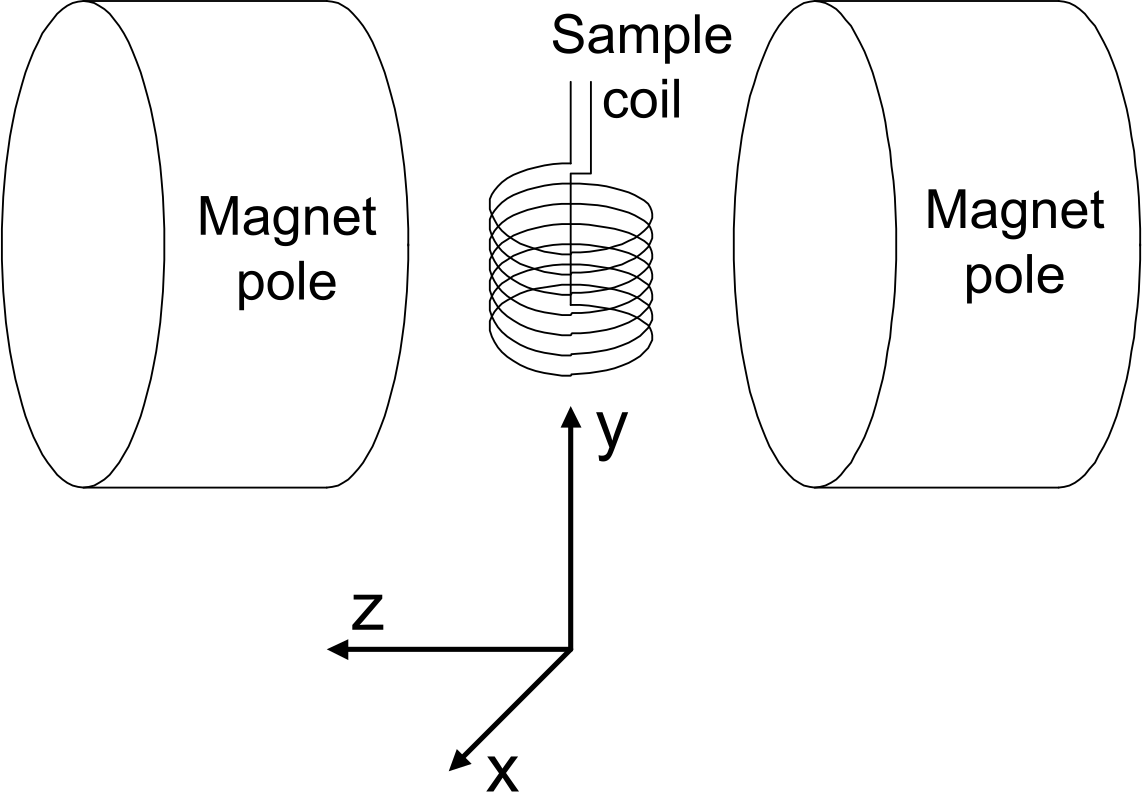
\includegraphics[width=0.8\textwidth]{magnet_aufbau.png}
    \captionof{figure}{Aufbau vom Magneten.\cite{TeachSpin}}
		\label{fig:alu}
	\end{Figure}

  Der \textbf{PS2 Controller} reguliert den Magneten auf die Raumtemperatur, um Imperfektionen/Inhomogenitäten zu reduzieren. Außerdem lässt er über die Stromzufuhr der Helmholzspulen dessen Gradienten einstellen. Dafür sind uns die Regler für $X$, $Y$, $Z$ und $Z^2$ gegeben. Diese sind später bei der Justage für $\frac{\pi}{2}$- bzw. $\pi$-Pulse iterativ zu optimieren. Zusätzslich lässt sich neben der Sträke auch das Vorzeichen der Gradienten mithilfe eines jeweiligen Schalters einstellen.

  Der \textbf{Mainframe} enthält einen Receiver, der ein einkommendes Signal zur Darstellung am Oszilloskop verstärken kann, einen Synthesizer, der die Frequenz des zirkular polarisierten Mangetfeldes angibt, einen Pulse Programmer, der zwei Pulse einstellen kann und diese periodeisch wieder gibt, wobei der Abstand der zwei Pulse unser $\tau$ ist. Außerdem gibt es noch ein Lock-In / Field Sweep, welchen wir aber nicht benötigen.

  Das digitale \textbf{Oszilloskop} kann dann unsere Signal darstellen. Dafür stehen uns drei Eingänge zur verfügung. 

  


\end{multicols}
\printbibliography

\end{document}
